% Requires: \usepackage{pgfplots}\pgfplotsset{compat=1.18}
% The bars are the paired accuracy GAIN from adding the insight to the bare
% problem (q -> q,i and q -> i,q), n = 1,000 items/model; labels give the gain
% in pp with McNemar stars.
% NB: legend entries are wrapped in { } so the comma inside $\{q,i\}$ is not
%     read as the pgfplots legend-entry separator.
\begin{figure}[t]
\centering
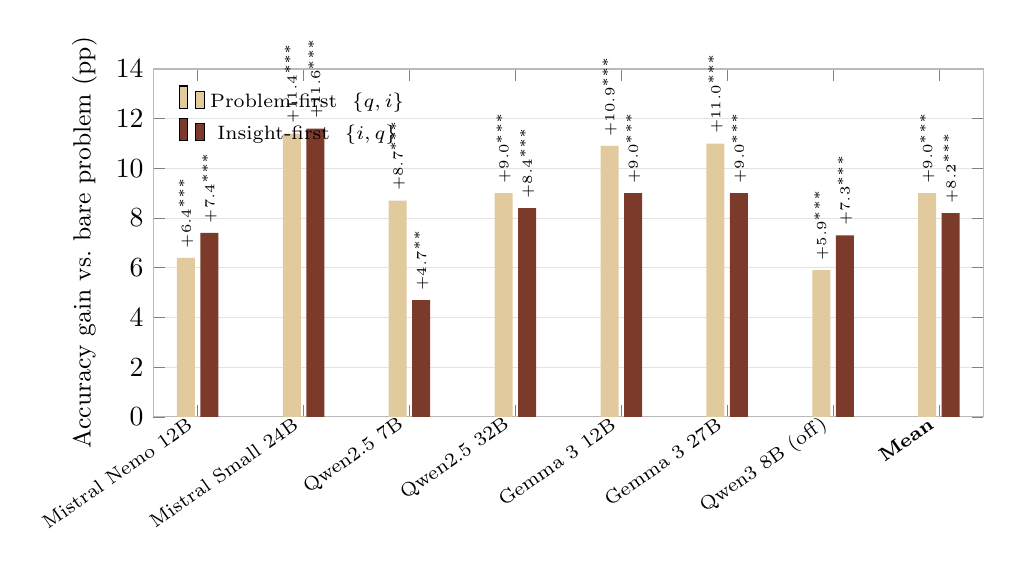
\begin{tikzpicture}
\begin{axis}[
    width=\columnwidth, height=6.0cm,
    ybar, bar width=6.5pt, enlarge x limits=0.06,
    ymin=0, ymax=14,
    ylabel={Accuracy gain vs.\ bare problem (pp)}, ylabel style={font=\small},
    symbolic x coords={Nemo12B, Mistral24B, Qwen7B, Qwen32B, Gemma12B, Gemma27B, Qwen8B, Mean},
    xtick=data,
    xticklabels={Mistral Nemo 12B, Mistral Small 24B, Qwen2.5 7B, Qwen2.5 32B,
                 Gemma 3 12B, Gemma 3 27B, Qwen3 8B (off), \textbf{Mean}},
    xticklabel style={rotate=35, anchor=east, font=\scriptsize},
    ytick={0,2,4,6,8,10,12,14}, ymajorgrids, grid style={gray!22}, tick align=inside,
    legend style={at={(0.02,0.97)}, anchor=north west, font=\scriptsize, draw=none, fill=none},
    nodes near coords, point meta=explicit symbolic,
    every node near coord/.append style={font=\tiny, rotate=90, anchor=west},
    axis line style={gray!55},
]
\addplot[draw=none, fill={rgb,255:red,226;green,202;blue,159}]  % problem-first q->{q,i}
  coordinates {(Nemo12B,6.4)[$+6.4^{\ast\ast\ast}$] (Mistral24B,11.4)[$+11.4^{\ast\ast\ast}$]
    (Qwen7B,8.7)[$+8.7^{\ast\ast\ast}$] (Qwen32B,9.0)[$+9.0^{\ast\ast\ast}$]
    (Gemma12B,10.9)[$+10.9^{\ast\ast\ast}$] (Gemma27B,11.0)[$+11.0^{\ast\ast\ast}$]
    (Qwen8B,5.9)[$+5.9^{\ast\ast\ast}$] (Mean,9.0)[$+9.0^{\ast\ast\ast}$]};
\addplot[draw=none, fill={rgb,255:red,123;green,58;blue,42}]    % insight-first q->{i,q}
  coordinates {(Nemo12B,7.4)[$+7.4^{\ast\ast\ast}$] (Mistral24B,11.6)[$+11.6^{\ast\ast\ast}$]
    (Qwen7B,4.7)[$+4.7^{\ast\ast}$] (Qwen32B,8.4)[$+8.4^{\ast\ast\ast}$]
    (Gemma12B,9.0)[$+9.0^{\ast\ast\ast}$] (Gemma27B,9.0)[$+9.0^{\ast\ast\ast}$]
    (Qwen8B,7.3)[$+7.3^{\ast\ast\ast}$] (Mean,8.2)[$+8.2^{\ast\ast\ast}$]};
\legend{{Problem-first\ \ $\{q,i\}$}, {Insight-first\ \ $\{i,q\}$}}
\end{axis}
\end{tikzpicture}
\caption{\textbf{The insight effect.} Paired accuracy gain from adding the retrieved
insight card to the bare problem, per model, over the same $n=1{,}000$ questions
(temp.\ 0.7, TRS prompt). Both placements help every one of the seven non-reasoning
models; labels give the gain in pp with McNemar significance
($^{\ast\ast\ast}p<.001$, $^{\ast\ast}p<.01$). The effect averages $+9.0$~pp
problem-first and $+8.2$~pp insight-first and is highly significant pooled across
models (Table~\ref{tab:pooled}); its magnitude dwarfs every composition effect
(ordering, repetition) studied in the rest of the paper.}
\label{fig:insight-effect}
\end{figure}
